\documentclass[11pt]{amsart}
\usepackage[a4paper,margin=0.9in]{geometry}
\usepackage[T1]{fontenc}
\usepackage[utf8]{inputenc}
\usepackage{lmodern,amsmath,amssymb,mathtools,microtype,booktabs,array}
\usepackage{xcolor,tikz,hyperref,etoolbox,needspace}
% Compact the AMS title whitespace while retaining 11pt body text.
\makeatletter
\patchcmd{\@maketitle}{\global\topskip42\p@}{\global\topskip24\p@}{}{}
\patchcmd{\@maketitle}{\dimen@34\p@}{\dimen@18\p@}{}{}
\patchcmd{\@setauthors}{\@topsep30\p@}{\@topsep18\p@}{}{}
\patchcmd{\@setabstracta}{\skip@20\p@}{\skip@12\p@}{}{}
\makeatother
\usetikzlibrary{arrows.meta,calc}
\definecolor{RelA}{HTML}{C44E00}
\definecolor{RelB}{HTML}{0067A5}
\definecolor{RelC}{HTML}{8B368C}
\definecolor{RelD}{HTML}{087A4B}
\newcommand{\Arel}{\textcolor{RelA}{A}}
\newcommand{\Brel}{\textcolor{RelB}{B}}
\newcommand{\Crel}{\textcolor{RelC}{C}}
\newcommand{\Drel}{\textcolor{RelD}{D}}
\newcommand{\Rrel}{R}
\newcommand{\restr}{\mathbin{\upharpoonright}}
\newcommand{\unsat}{\mathsf{unsat}}
\newtheorem{theorem}{Theorem}
\newtheorem{lemma}[theorem]{Lemma}
\newtheorem{proposition}[theorem]{Proposition}
\hypersetup{colorlinks=true,linkcolor=black,citecolor=black,urlcolor=RelB,
 pdftitle={Four Well-Founded Relations: A Sufficient Rule, an Infinite Counterexample, and a Finite Bound},
 pdfauthor={Nachum Dershowitz}}
\pdfstringdefDisableCommands{\def\Arel{A}\def\Brel{B}\def\Crel{C}\def\Drel{D}\def\Rrel{R}}
\setlength{\textfloatsep}{12pt plus 2pt minus 2pt}
\setlength{\floatsep}{10pt plus 2pt minus 2pt}
\setlength{\intextsep}{10pt plus 2pt minus 2pt}
\title[Four Well-Founded Relations]{Four Well-Founded Relations: A Sufficient Rule, an Infinite Counterexample, and a Finite Bound}
\author{Nachum Dershowitz}
\address{School of Computer Science and AI, Tel Aviv University, Tel Aviv, Israel}
\date{}

\begin{document}
\begin{abstract}
A four-relation instance of preferential jumping gives a sufficient condition for the union of four well-founded relations. The proposed alternative to its last condition fails: a countable example satisfies all three alternative conditions, even with short detours, while its union has a two-cycle. The counterexample is formally verified in Rocq. An exact SMT enumeration excludes finite examples of this kind on at most ten points. We give the construction, the normal forms and encoding required for the finite claim, and references to the accompanying formal proofs, generators, and run tables.
\end{abstract}
\maketitle

\section{The Two Rules}
A binary relation \(P\) on a set \(X\) is a subset of \(X\times X\); we write \(xPy\) for \((x,y)\in P\), calling this a directed edge from \(x\) to its \(P\)-successor \(y\). Composition is read left to right: \(xPQz\) means \(xPyQz\) for some \(y\in X\). A finite \(P\)-path from \(x\) to \(z\) is a sequence \(x=x_0,x_1,\ldots,x_m=z\) with \(x_iPx_{i+1}\) for every \(i<m\). Its length is \(m\). Thus \(P^m\) relates the endpoints of paths of length exactly \(m\), \(P^+\) those of positive length, and \(P^*\) those of any finite length, including zero. In particular, \(P^0\) is the identity relation and \(P^2=PP\).

A relation is \emph{well-founded} here if it admits no infinite forward chain \(x_0Px_1Px_2P\cdots\). Unions allow an edge of any of their constituent relations, and \(P\subseteq Q\) means that every \(P\)-edge is a \(Q\)-edge. Throughout, \(\Arel,\Brel,\Crel,\Drel\) are individually well-founded relations on the same set, and
\[
 \Rrel=\Arel\cup\Brel\cup\Crel\cup\Drel.
\]

\begin{theorem}[Dawson--Dershowitz--Gor\'e]\label{thm:positive}
The union \(\Rrel\) is well-founded under the conditions
\begin{align}
 (\Brel\cup\Crel\cup\Drel)\Arel
 &\subseteq \Arel\Rrel^*\cup\Brel\cup\Crel\cup\Drel,\tag{P0}\label{P0}\\
 (\Crel\cup\Drel)\Brel
 &\subseteq \Arel\Rrel^*\cup\Brel^+\cup\Crel\cup\Drel,\tag{P1}\label{P1}\\
 \Drel\Crel
 &\subseteq \Crel(\Crel\cup\Drel)^*\cup\Drel.\tag{P2}\label{P2}
\end{align}
Every finite \(\Rrel\)-path can moreover be replaced, with the same endpoints, by a path in \(\Arel^*\Brel^*\Crel^*\Drel^*\): a block of \(\Arel\)-edges followed by blocks of \(\Brel\)-, \(\Crel\)-, and \(\Drel\)-edges, any of which may be empty.
\end{theorem}
This is the four-relation case of the Preferential Jumping theorem in \cite[Theorem~28]{DDG}, with the path-rearrangement conclusion of \cite[Theorem~29]{DDG}. (The proof in \cite{DDG} was machine checked in Isabelle/HOL.) Condition \eqref{P2} first establishes well-foundedness of \(\Crel\cup\Drel\); \eqref{P1} and \eqref{P0} then incorporate \(\Brel\) and \(\Arel\).

Each inclusion prescribes a \emph{repair path}: an alternative finite path with the same starting and ending points as the two-edge path on the left. For example, if \(x(\Brel\cup\Crel\cup\Drel)y\Arel z\), condition \eqref{P0} requires either a path \(x\Arel u\Rrel^*z\), for some \(u\), or a single \((\Brel\cup\Crel\cup\Drel)\)-edge from \(x\) to \(z\). A repair changes the intermediate route, not the endpoints; its edges must already belong to the given relations.

The question posed in \cite[\S9]{DDG} is whether the well-foundedness conclusion remains true if \eqref{P0} and \eqref{P1} are retained but \eqref{P2} is replaced by
\begin{equation}
 \Drel\Crel\subseteq \Brel(\Brel\cup\Crel\cup\Drel)^*\cup\Crel^+\cup\Drel.\tag{Q2}\label{Q2}
\end{equation}
Here a \(\Drel\Crel\)-path may instead be repaired by a \(\Brel\)-edge followed by any finite path using \(\Brel,\Crel,\Drel\), by a nonempty \(\Crel\)-path, or by one \(\Drel\)-edge. The next construction gives a negative answer to this proposed replacement.

\section{A Countable Counterexample}
\begin{theorem}\label{thm:counterexample}
Conditions \eqref{P0}, \eqref{P1}, and \eqref{Q2} do not imply well-foundedness of \(\Rrel\), even when their respective right sides are strengthened to
\(\Arel(\Crel\cup\Drel)\cup\Crel\cup\Drel\), \(\Brel^2\cup\Arel\Brel^2\), and \(\Brel\Drel\).
\end{theorem}
\begin{proof}
Let \(X=\mathbb N\uplus\{p,q\}\), with \(\mathbb N=\{0,1,\ldots\}\), and take exactly these edges, for \(k\geq0\):
\begin{equation}\label{eq:edges}
\begin{array}{c|l}
 \Arel & 2k\,\Arel\,q,\quad (2k+1)\,\Arel\,p\\
 \Brel & p\,\Brel\,(2k),\quad q\,\Brel\,(2k+1),\quad (k+1)\,\Brel\,k\\
 \Crel & q\,\Crel\,p\\
 \Drel & p\,\Drel\,q,\quad 0\,\Drel\,p.
\end{array}
\end{equation}
Figure~\ref{fig:counterexample} displays these edges and the repeating natural-number part of the construction. Neither \(\Arel\) nor \(\Crel\) admits two consecutive steps, so \(\Arel^2=\Crel^2=\varnothing\). The longest \(\Drel\)-path is \(0\Drel p\Drel q\), so \(\Drel^3=\varnothing\). A \(\Brel\)-path from \(p\) or \(q\) first chooses a natural number; every subsequent step decreases it by one. Thus \(\Brel\) also has no infinite chain. Equivalently, its edges decrease the ordinal rank \(\rho(p)=\rho(q)=\omega\), \(\rho(n)=n\), where \(\omega\) exceeds every natural number. Nevertheless, the two edges between \(p\) and \(q\) in Figure~\ref{fig:counterexample} give the infinite \(\Rrel\)-chain \(p\Drel q\Crel p\Drel q\Crel p\cdots\).

\begin{figure}[t]
\centering
% Full-width vector drawing; the same named colors are used in the paper.
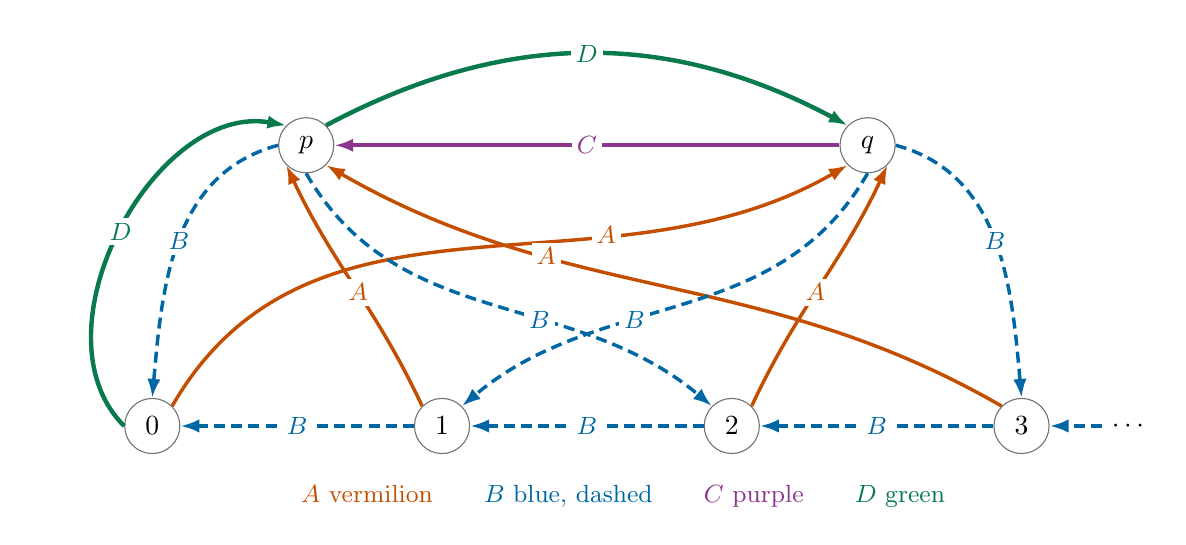
\begin{tikzpicture}[x=1.15cm,y=1.15cm,
 vertex/.style={circle,draw=black!55,fill=white,minimum size=7mm,inner sep=0pt,font=\normalsize},
 edge/.style={-{Latex[length=2.4mm,width=1.7mm]},line width=1.25pt},
 edgeA/.style={edge,draw=RelA},
 edgeB/.style={edge,draw=RelB,dash pattern=on 4pt off 2.2pt},
 edgeC/.style={edge,draw=RelC,line width=1.6pt},
 edgeD/.style={edge,draw=RelD,line width=1.6pt},
 lab/.style={fill=white,inner sep=1.8pt,font=\small}]
\node[vertex] (p) at (-3.1,3.1) {$p$};
\node[vertex] (q) at (3.1,3.1) {$q$};
\node[vertex] (n0) at (-4.8,0) {$0$};
\node[vertex] (n1) at (-1.6,0) {$1$};
\node[vertex] (n2) at (1.6,0) {$2$};
\node[vertex] (n3) at (4.8,0) {$3$};
\node (more) at (6.0,0) {$\cdots$};

% Long crossing edges run at separate heights. All crossings are unmarked.
\draw[edgeA] (n0.north east) to[out=60,in=210] node[lab,pos=.68] {$\Arel$} (q.south west);
\draw[edgeA] (n3.north west) to[out=150,in=330] node[lab,pos=.68] {$\Arel$} (p.south east);
\draw[edgeB] (p.south) to[out=300,in=140] node[lab,pos=.61] {$\Brel$} (n2.north west);
\draw[edgeB] (q.south) to[out=240,in=40] node[lab,pos=.61] {$\Brel$} (n1.north east);

% Short A edges and the two outer B edges.
\draw[edgeA] (n1.north west) to[out=115,in=295] node[lab,pos=.47] {$\Arel$} (p.south west);
\draw[edgeA] (n2.north east) to[out=65,in=245] node[lab,pos=.47] {$\Arel$} (q.south east);
\draw[edgeB] (p.west) to[out=195,in=85] node[lab,pos=.50] {$\Brel$} (n0.north);
\draw[edgeB] (q.east) to[out=-15,in=95] node[lab,pos=.50] {$\Brel$} (n3.north);

% The natural-number descent and the extra D edge.
\draw[edgeB] (n1.west) -- node[lab] {$\Brel$} (n0.east);
\draw[edgeB] (n2.west) -- node[lab] {$\Brel$} (n1.east);
\draw[edgeB] (n3.west) -- node[lab] {$\Brel$} (n2.east);
\draw[edgeB] (more.west) -- (n3.east);
\draw[edgeD] (n0.west) to[out=135,in=170] node[lab,pos=.50] {$\Drel$} (p.north west);

% The cycle is visually isolated above the infinite family of edges.
\draw[edgeD] (p.north east) to[out=28,in=152] node[lab,pos=.5] {$\Drel$} (q.north west);
\draw[edgeC] (q.west) -- node[lab,pos=.5] {$\Crel$} (p.east);

\node[anchor=north,font=\small,align=center] at (.4,-.55)
 {$\textcolor{RelA}{\Arel\ \text{vermilion}}\qquad
   \textcolor{RelB}{\Brel\ \text{blue, dashed}}\qquad
   \textcolor{RelC}{\Crel\ \text{purple}}\qquad
   \textcolor{RelD}{\Drel\ \text{green}}$};
\end{tikzpicture}

\caption{The countable counterexample, with exactly the edges in \eqref{eq:edges}. The natural-number row and the alternating families of \(\Arel\)- and \(\Brel\)-edges continue indefinitely; the dashed \(\Brel\)-edges include every downward step \((k+1)\Brel k\). The upper pair \(p\Drel q\Crel p\) forms the cycle. Colors match the relation names throughout the paper.}
\label{fig:counterexample}
\end{figure}

Write \(a(n)=q\) for even \(n\) and \(a(n)=p\) for odd \(n\). Then \(n\Arel a(n)\) and \(a(n+1)(\Crel\cup\Drel)a(n)\). Since only natural numbers have outgoing \(\Arel\)-edges and every \(\Crel\)- or \(\Drel\)-edge ends at \(p\) or \(q\), a \((\Brel\cup\Crel\cup\Drel)\Arel\)-path must begin with \(\Brel\). Its three possible forms have the following repairs; \(\rightsquigarrow\) separates a path from its replacement with the same endpoints:
\begin{align*}
 p\Brel 2k\Arel q &\rightsquigarrow p\Drel q,\\
 q\Brel(2k+1)\Arel p &\rightsquigarrow q\Crel p,\\
 (n+1)\Brel n\Arel a(n)
 &\rightsquigarrow (n+1)\Arel a(n+1)(\Crel\cup\Drel)a(n).
\end{align*}
Hence \((\Brel\cup\Crel\cup\Drel)\Arel\subseteq\Arel(\Crel\cup\Drel)\cup\Crel\cup\Drel\).
The three types of \((\Crel\cup\Drel)\Brel\)-path have endpoint-preserving repairs
\begin{align*}
 p\Drel q\Brel(2k+1)&\rightsquigarrow p\Brel(2k+2)\Brel(2k+1),\\
 q\Crel p\Brel(2k)&\rightsquigarrow q\Brel(2k+1)\Brel(2k),\\
 0\Drel p\Brel(2k)&\rightsquigarrow 0\Arel q\Brel(2k+1)\Brel(2k).
\end{align*}
Thus \((\Crel\cup\Drel)\Brel\subseteq\Brel^2\cup\Arel\Brel^2\). Finally \(\Drel\Crel=\{(p,p)\}\subseteq\Brel\Drel\), witnessed by \(p\Brel0\Drel p\). These stronger inclusions imply \eqref{P0}, \eqref{P1}, and \eqref{Q2}.
\end{proof}
The use of infinitude is in the first two \((\Crel\cup\Drel)\Brel\) repairs: the \(\Brel\)-edge into \(n\) is reached from \(n+1\). A truncation at its largest integer loses one of these repairs. Repair paths nevertheless have at most three edges.

\smallskip
\begin{samepage}
\noindent\textbf{Formal verification.}
The file \texttt{FourRelationsCounterexample.v} formalizes Theorem~\ref{thm:counterexample}: individual well-foundedness, the three stronger inclusions, and nontermination via the explicit chain \(p,q,p,q,\ldots\). Compilation in Rocq~9.1.1 and the independent \texttt{rocq check} verifier both succeed. The proofs use only the standard library, with no axioms or unfinished proofs; \texttt{Print Assumptions} reports ``Closed under the global context.'' These formal proofs and their verification record are in the companion archive~\cite{archive}, under \texttt{formal\_proofs/}.
\par\end{samepage}

\section{Normal Forms for a Finite Search}
We first specify the terminology used in the finite search. For a subset \(Y\subseteq X\), the restriction \(P\restr Y\) keeps exactly those \(P\)-edges with both endpoints in \(Y\). A point \(x\in Y\) is \emph{\(P\)-minimal in \(Y\)} if there is no \(y\in Y\) with \(xPy\). 
%A relation is \emph{acyclic} if it has no positive-length path from a point to itself. 
%A relation is \emph{strongly connected} if every pair of points is mutually reachable by finite paths. 
%A \emph{strongly connected component} is a maximal set with this property; it is a \emph{sink} component if no edge leaves it. 
A {strongly connected component} is a \emph{sink} if no edge leaves it. 
A \emph{simple cycle} repeats no vertex other than its first vertex at the end, and it is \emph{chordless} if there is no edge between its vertices other than its cycle edges.
On a finite set, acyclicity is equivalent to well-foundedness. 

For any relation \(P\), let \(P^\infty\) be the set of points beginning an infinite forward \(P\)-chain.
Restriction to \(I=\Rrel^\infty\) preserves the interaction conditions: every intermediate point on a repair path ending in \(I\) can follow the rest of that path and then an infinite \(\Rrel\)-chain, so it also belongs to \(I\). In a counterexample \(I\) is nonempty. Define
\[
 S_A=\{x\in I:\neg\exists y\in I.\;x\Arel y\},\qquad
 S_B=\{x\in S_A:\neg\exists y\in S_A.\;x\Brel^+y\}.
\]
Thus \(S_A\) consists of the \(\Arel\)-minimal points of \(I\), and \(S_B\) consists of the \(\Brel^+\)-minimal points of \(S_A\). Both are nonempty since \(\Arel\) and \(\Brel^+\) are well-founded.

\begin{lemma}[Surviving tail]\label{lem:tail}
Under \eqref{P0}--\eqref{P1}, every \(x\in S_B\) has a \((\Crel\cup\Drel)\)-successor in \(S_B\). Under \eqref{Q2}, the subrelation of \(\Crel\cup\Drel\) formed by keeping only sources without a \(\Brel\)-successor in \((\Brel\cup\Crel\cup\Drel)^\infty\) is well-founded.
\end{lemma}
\begin{proof}
The iterated inclusions
\begin{align*}
 (\Brel\cup\Crel\cup\Drel)\Arel^*
 &\subseteq\Arel\Rrel^*\cup\Brel\cup\Crel\cup\Drel,\\
 (\Crel\cup\Drel)\Brel^+
 &\subseteq\Arel\Rrel^*\cup\Brel^+\cup\Crel\cup\Drel
\end{align*}
follow by induction on path length. For \(x\in S_A\), choose an \(\Arel\)-minimal \((\Brel\cup\Crel\cup\Drel)\)-successor within \(I\). If it had an \(\Arel\)-successor, \eqref{P0} would give either an \(\Arel\)-edge from \(x\) or a smaller \((\Brel\cup\Crel\cup\Drel)\)-successor. Thus it lies in \(S_A\). For \(x\in S_B\) this edge must be in \(\Crel\cup\Drel\). Choose a \(\Brel^+\)-minimal \((\Crel\cup\Drel)\)-successor in \(S_A\). If it were outside \(S_B\), the second iterated inclusion would give an \(\Arel\)-edge from \(x\), a \(\Brel^+\)-path from \(x\) into \(S_A\), or a smaller \((\Crel\cup\Drel)\)-successor, all impossible.

For the last assertion apply the detour lemma of \cite[\S4, Lemma~25]{DDG} to \(P=\Crel\), \(Q=\Drel\), \(U=\Brel\), \(S=\Brel\cup\Crel\cup\Drel\). Its premise is \eqref{Q2}. Restricting \(\Drel\) to sources without a \(\Brel\)-successor in \((\Brel\cup\Crel\cup\Drel)^\infty\) preserves well-foundedness, so the lemma gives well-foundedness of the same restriction of \(\Crel\cup\Drel\).
\end{proof}

\begin{proposition}[Finite normal form]\label{prop:normal}
If a finite counterexample exists, one of minimum cardinality can be labeled \(X_n=\{0,\ldots,n-1\}\) so that \(\Rrel\) is strongly connected; all \(\Arel\)-edges descend in label; \(S_A=[0,s_0)\) and \(S_B=[0,s_1)\), where \([0,s)=\{0,\ldots,s-1\}\); and \(0,\ldots,L-1\) are a shortest simple \((\Crel\cup\Drel)\restr S_B\)-cycle in cyclic order. The selected cycle is chordless and admits an edge coloring using both \(\Crel\) and \(\Drel\). For \(L=2\) it has the form \(0\Drel1\Crel0\), with \(0\Brel v(\Brel\cup\Crel\cup\Drel)^*0\) for some \(v\notin S_A\).
\end{proposition}
\begin{proof}
Restrict to \(I\) and choose a sink strongly connected component of \(\Rrel\). All repair witnesses remain inside this closed component, which contains a cycle; minimality makes it all of \(X_n\). Since \(\Arel\) is acyclic, its vertices can be numbered so that every \(\Arel\)-edge goes from a larger number to a smaller one. This is a topological ordering with sinks first. It can put the \(\Arel\)-minimal set \(S_A\) first, with \(S_B\) first within it.

Lemma~\ref{lem:tail} supplies the \((\Crel\cup\Drel)\)-cycle. A chord would shorten a shortest cycle; an all-\(\Crel\) or all-\(\Drel\) cycle contradicts individual acyclicity. In length two the two colors are forced. Apply \eqref{Q2} to \(0\Drel1\Crel0\): the \(\Crel^+\) and \(\Drel\) repairs give monochromatic cycles, leaving \(0\Brel v(\Brel\cup\Crel\cup\Drel)^*0\). If \(v\in S_A\), this contradicts \(0\in S_B\).
\end{proof}
The same tripartite theorem from \cite{DDG} shows that \(\Arel\cup\Brel\) has a cycle in every finite counterexample: apply it to \(\Arel\cup\Brel,\Crel,\Drel\) if the first union were acyclic. Lemma~\ref{lem:tail} gives the other necessary cycle, in \(\Crel\cup\Drel\).

\smallskip
\noindent\textbf{Reduction to an exact size.}
A counterexample on at most \(n\) points yields a strongly connected one on exactly \(n\) points. First take a minimum counterexample and its cyclic strongly connected component as above. Choose a surjection \(f:V\to W\) from an \(n\)-element set onto that component, and lift each relation by
\[
 uP'v\quad\Longleftrightarrow\quad f(u)P f(v),
 \qquad P\in\{\Arel,\Brel,\Crel,\Drel\}.
\]
A monochromatic cycle upstairs would project to one downstairs, so the four lifted relations remain acyclic. Every repair is a positive-length labeled path and lifts between any prescribed preimages of its endpoints; hence the interaction conditions persist. Every pair of points of the cyclic component, including a point paired with itself, is joined by a positive-length path. These paths lift as well, so the new union is strongly connected and cyclic. The same labeling and shortest-cycle normalizations therefore apply at size \(n\).

\section{Exact Exclusion Through Ten Points}
The search uses satisfiability modulo theories (SMT): it asks whether Boolean edge variables can satisfy all the stated constraints. A result of \(\unsat\) means that no assignment satisfies that branch. For \(P\in\{\Arel,\Brel,\Crel,\Drel\}\) and \(i,j<n\), let \(P_{ij}\) be true exactly when \(iPj\). Unions are disjunctions, \((PQ)_{ij}=\bigvee_{k<n}(P_{ik}\land Q_{kj})\), and closure is computed exactly by
\begin{gather*}
 T^{(-1)}_{ij}=(i=j)\lor P_{ij},\qquad
 T^{(k)}_{ij}=T^{(k-1)}_{ij}\lor\bigl(T^{(k-1)}_{ik}\land T^{(k-1)}_{kj}\bigr),\\
 P^*_{ij}=T^{(n-1)}_{ij},\qquad P^+_{ij}=\bigvee_k P_{ik}\land P^*_{kj}.
\end{gather*}
Here \(T^{(k)}\) records reachability allowing intermediate vertices only among \(0,\ldots,k\), and every disjunction ranges over the \(n\) vertices. The recurrence therefore computes the full finite closures, not an approximation by a fixed path length.
The Boolean-matrix and row-wise bit-vector generators assert acyclicity of each color, a cycle of \(\Rrel\) and of \(\Arel\cup\Brel\), all three inclusions, and the normal forms above. Strong connectivity makes \(\Arel\Rrel^*\) the full row exactly when the corresponding \(\Arel\) row is nonempty. The restricted \(\Crel\cup\Drel\) relation from Lemma~\ref{lem:tail} is asserted acyclic using \((\Brel\cup\Crel\cup\Drel)\)-cycle reachability; \(S_A,S_B\) are defined by the exact rows of \(\Arel,\Brel^+\), respectively. These are necessary constraints on every smallest finite counterexample.

The generators enumerate the selected shortest cycle, its witnessed colors and the canonical \(s_0,s_1\) sizes. Length \(L=n\) is impossible: \(S_A=X_n\) makes \(\Arel\) empty, contradicting the necessary \(\Arel\cup\Brel\)-cycle. For \(L=2\), the \(\Brel(\Brel\cup\Crel\cup\Drel)^*\) witness, its least \(\Arel\)-successor and the \((\Crel\cup\Drel)\Brel\) repair are split explicitly. The last two residual branches are closed by whole-branch SMT calls, with returning witnesses \(v=7,8\) and least \(\Arel\)-successors \(a=3,4\), respectively. Their exact inputs, solver outputs, parameters, and timings are included in the archive~\cite{archive}.

\begin{table}[t]
\centering
\small
\setlength{\tabcolsep}{4pt}
\begin{tabular}{@{}llr@{}}
\toprule
Domain and family & Exhaustive completed branches & \(\unsat\)\\
\midrule
\(n=9,\ L=2,3,4,5..8\) & \(28+42+60+20\) & 150\\
\(n=10,\ L=3..9\) & Canonical cycle branches & 280\\
\(n=10,\ L=2\) & Initial, refined, residual, final branches & \(32+240+18+2=292\)\\
\bottomrule
\end{tabular}
\caption{Completed finite searches. Four unresolved ten-point root cases split into 260 branches (240 closed), leaving 20 residual cases. Eighteen close in the residual table; two final whole-branch runs close the remainder. Thus the ten-point cover has \(280+292=572\) terminal UNSAT cases. Smaller sizes follow by the exact-size reduction.}
\label{tab:runs}
\end{table}

\Needspace{15\baselineskip}
\begin{theorem}\label{thm:finite}
No counterexample to \eqref{P0}, \eqref{P1}, \eqref{Q2} on at most ten points exists.
\end{theorem}
\begin{proof}
If a counterexample existed on at most ten points, the exact-size reduction would give a strongly connected one on exactly ten points. Applying the labeling and cycle normalizations of Proposition~\ref{prop:normal} would make one of the encoded branches satisfiable. Every branch in the exhaustive ten-point cover instead returns \(\unsat\). The archive checker, \texttt{verification/verify\_results.py}, reproduces a cover of 316 root cases: 312 close directly, four split into 260 refinements, 240 of these close directly, 18 close in the residual table, and the last two close in the saved whole-branch runs. This gives \(312+240+18+2=572\) terminal cases and no unresolved cases. The separate nine-point cover has 150 cases, all recorded as \(\unsat\).
\end{proof}

\section{Formalizations}

The companion archive~\cite{archive} contains the Rocq proofs, the finite encoders and result tables, the two final exact SMT inputs and outputs, and the coverage checker. The checker verifies the root and refinement partitions, saved outcomes, exit codes, and byte-for-byte regeneration and hashes of the final inputs. The finite bound is computer-assisted: its computational premises are the encoders and recorded solver results, rather than independently checked Z3 proof certificates. The Rocq proof of Theorem~\ref{thm:counterexample} is independent of this enumeration.

The following commands, run from the archive root, reproduce the finite-coverage audit using Python's standard library and then compile and independently check the counterexample development with Rocq:
\begin{quote}\ttfamily
python3 verification/verify\_results.py\\
sh formal\_proofs/check.sh
\end{quote}
The archive README gives the saved solver versions and the commands for rerunning the two final SMT inputs.

\section*{Acknowledgment}
The author acknowledges assistance from ChatGPT and Codex (OpenAI) with the Rocq formalization, checking the archived computations, and preparing the text and figure.

% Keep the short bibliography and author affiliation on the closing page.
\enlargethispage{2\baselineskip}
\begin{thebibliography}{2}
\bibitem{DDG}
J.~Dawson, N.~Dershowitz, and R.~Gor\'e, ``Well-Founded Unions,'' in \emph{Automated Reasoning (IJCAR 2018)}, Lecture Notes in Artificial Intelligence 10900, Springer, 2018, pp.~117--133.
\bibitem{archive}
N.~Dershowitz, \emph{Four Relations: Companion Archive}, release v1.0.0, 2026.
Rocq formalization and finite-search evidence.
\href{https://github.com/NachumDershowitz/4Relations/releases/tag/v1.0.0}{\nolinkurl{github.com/NachumDershowitz/4Relations}}, release v1.0.0.
\end{thebibliography}
\end{document}
